% -*- mode : latex; coding: utf-8 -*-
\chapter{CXLmem Design} \label{sec:CXLmem Design}

In this section, I used some new terminologies. MXP stands for memory expander connected via CXL interconnect which is equal to CXL type 3 device. DIMM means local DRAM memory which is connected to DIMM pins on processor. To timing simulate MXP and compare the performance of MXP to DIMM's performance, I implemented CXL type 3 device simulator \textit{CXLmem} using C++. CXLmem is trace-driven cycle-accurate simulator. Figure \ref{fig:cxlmem_design} shows the high level design of CXLmem.

\begin{figure}[ht]
  \centering
  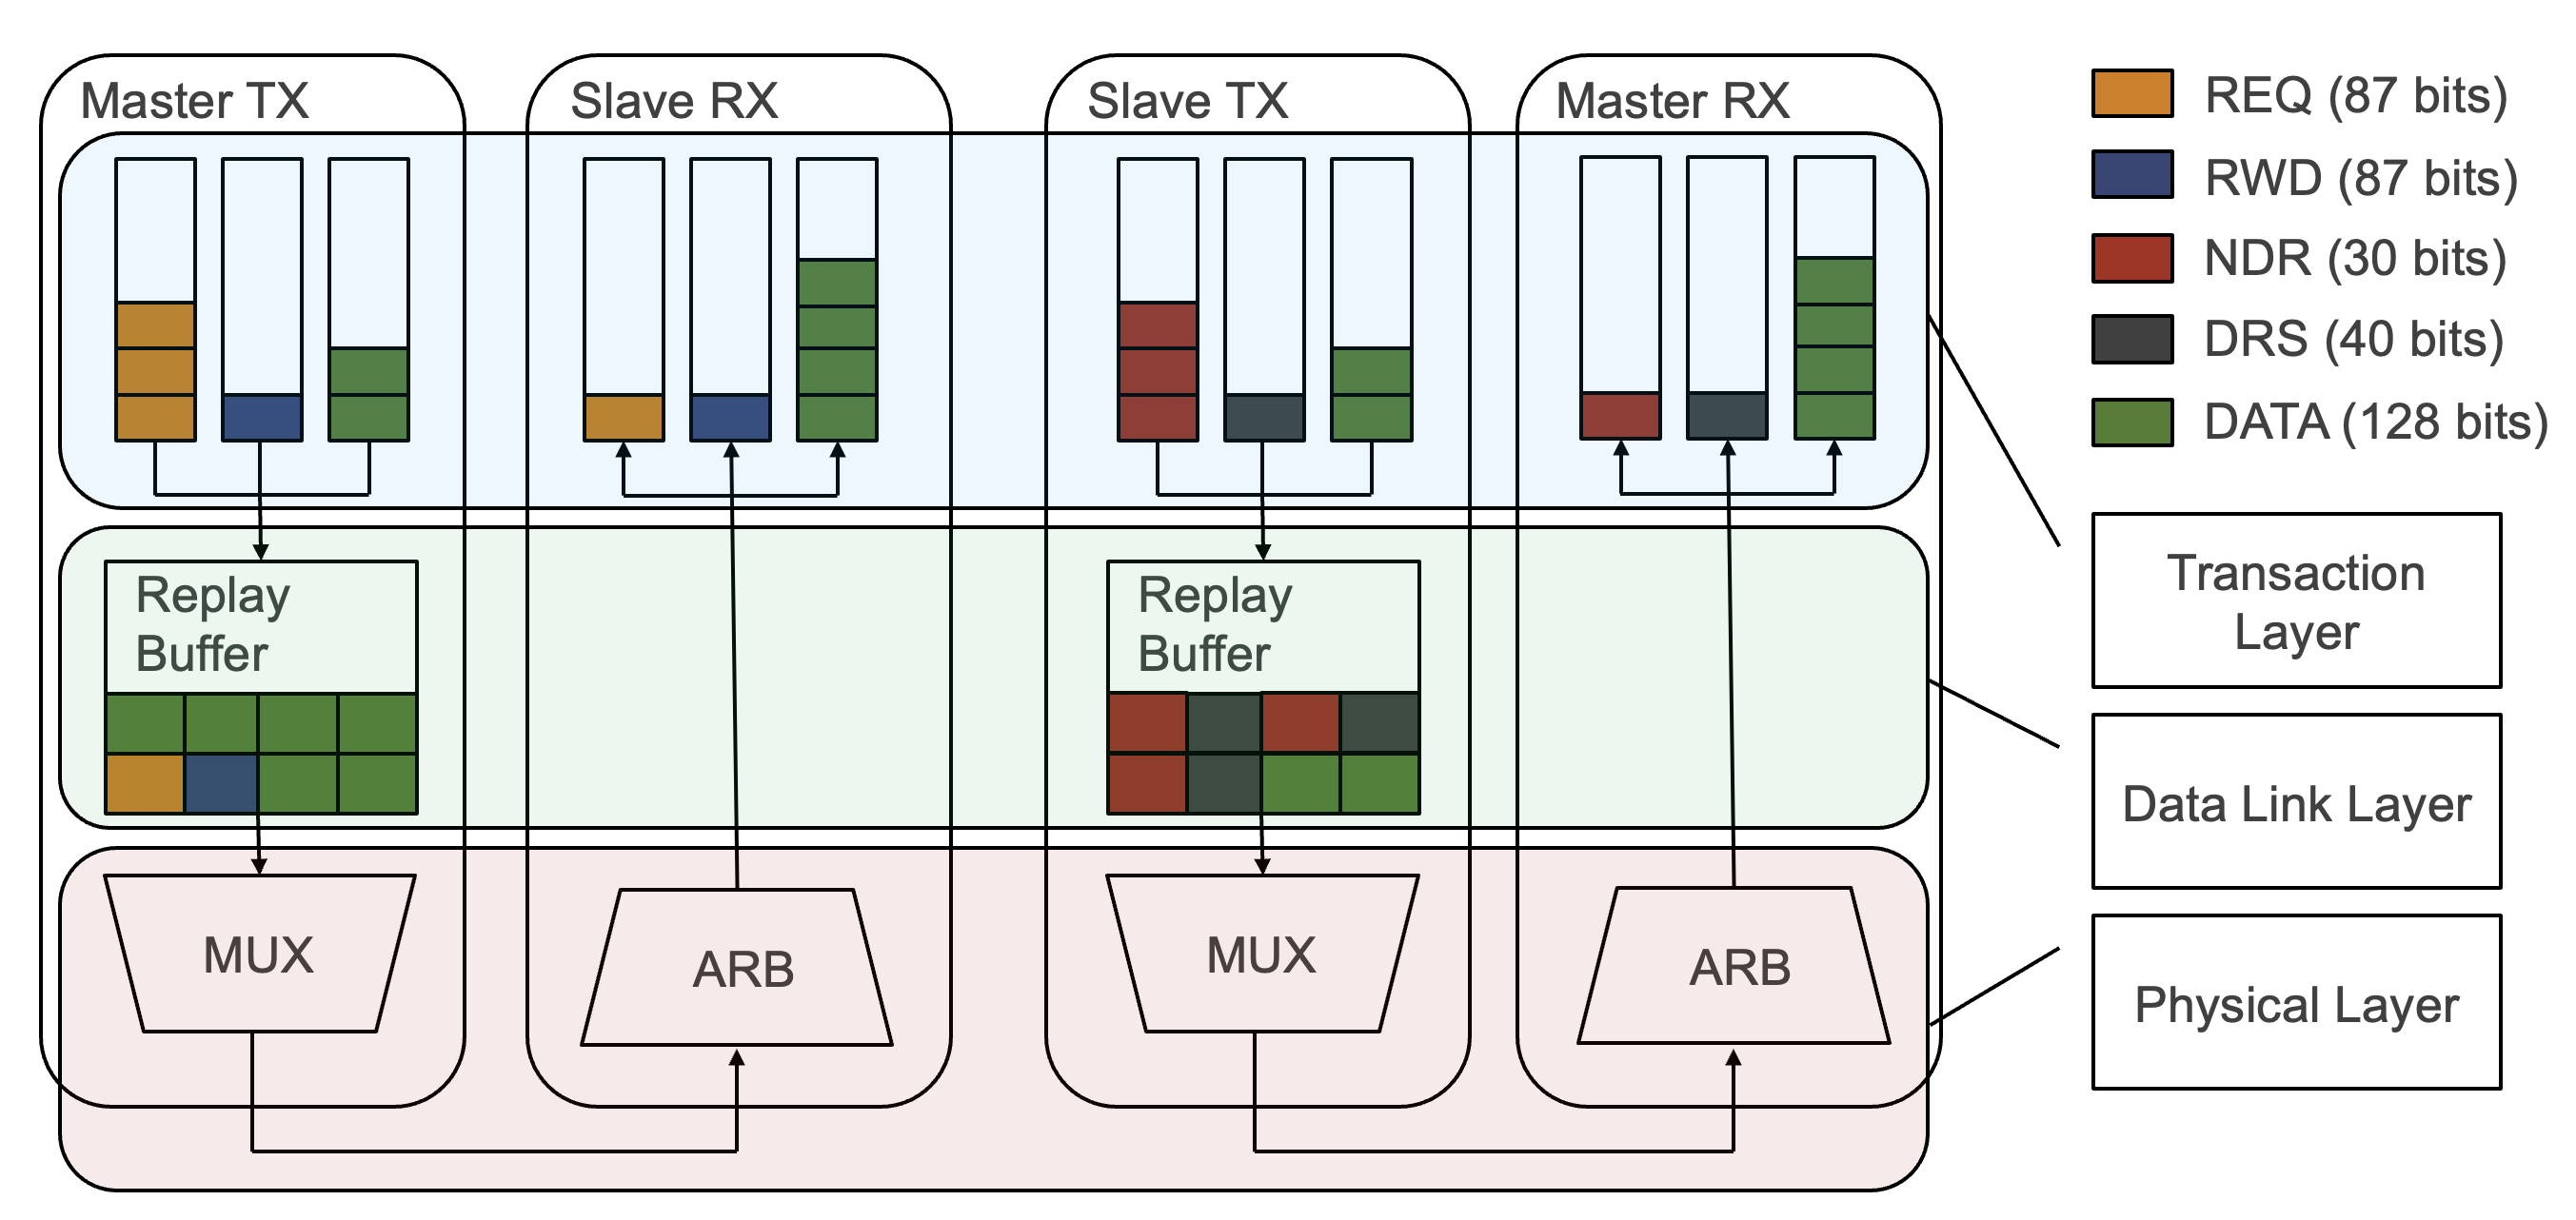
\includegraphics[width=\textwidth]{figures/cxlmem_design.png}
  \caption{High level design of CXLmem.}
  \label{fig:cxlmem_design}
\end{figure}

Both master and slave contain CXL endpoint module. In this research, master is CPU that sends memory requests to MXP and slave is MXP that responds to memory requests. Each CXL endpoint module has three layers (Transaction layer, Data link layer, Physical layer) of CXL.mem protocol. All the MXP memory requests and responds go through TX's (transmitter's) three layers in the order of transaction layer, data link layer, physical layer and RX's (receiver's) three layers in the order of physical layer, data link layer, physical layer. When TX wants to send a message, TX pushes the request or respond to \textit{pending queue} of CXL endpoint module. Then TX's transaction layer starts transaction of that message. After flit packing, TX sends flits to \textit{RX queue} that stores the received flits. At the end of transaction, RX's transaction layer pushes the received message to \textit{done queue}. All transaction through CXL interconnection starts at \textit{pending queue} on TX and ends at \textit{done queue} on RX. Now I will explain each layer's design in detail following the sequence of transaction.

\section{TX Transaction Layer} \label{sec:tx transaction layer}
TX's transaction layer reads \textit{pending queue} and moves the messages in \textit{pending queue} to appropriate virtual channel buffer. While virtual channel buffer has enough free space, transaction layer reads messages up to predefined threshold.

There are three Virtual channel buffers in transaction layer. Those are ``non-data'', ``with-data'', ``data''. Non-data virtual channel buffer stores REQ(master) or NDR(slave). Both REQ from master and NDR from slave contains no data. This non-data virtual channel buffer corresponds to the left most buffer in transaction layer in the Figure \ref{fig:cxlmem_design}. With-data virtual channel buffer stores RWD(master) or DRS(slave). Both RWD from master and DRS from slave bring data with those headers. This with-data virtual channel buffer corresponds to the buffer in the middle of transaction layer in the Figure \ref{fig:cxlmem_design}. Data virtual channel buffer stores only data that RWD(master) or DRS(slave) brings. This data virtual channel buffer corresponds to the right most buffer in transaction layer in the Figure \ref{fig:cxlmem_design}. The capacity of each virtual channel buffer can be configured separately.

If \textit{pending queue} contains non-data message, transaction layer checks the free space in non-data virtual channel buffer. When there's free space, transaction layer moves the messages to non-data virtual channel buffer. In contrast, if \textit{pending queue} has with-data message, transaction layer checks both free space in with-data virtual channel buffer and free space in data virtual channel buffer. Only when both virtual channel buffer have enough free space, transaction layer moves the messages to virtual channel buffers.

The timing parameters in TX's transaction layer are maximum number of messages to move from \textit{pending queue}, virtual channel size and virtual channel buffer push latency. Those can be configured easily to test diverse situations.

\section{TX Data Link Layer} \label{sec:tx data link layer}
TX's data link layer reads virtual channel buffers and create flits to send to RX. First, TX's data link layer checks free space in RX's virtual channel buffer. TX can create flits that are able to be stored in RX's virtual channel buffer. 

After checking free space in RX's virtual channel buffer, TX data link layer generates header slot first. Only when header slot is successfully generated, data link layer generates generic slots. Among messages in virtual channel buffers, data messages whose with-data message has already been sent, have higher priority. Because the with-data message's transaction can be finalized only when the all of corresponding data have already been arrived. Otherwise, with-data messages will occupy virtual channel buffer for long time, suppress other with-data message transaction. This will lead to degradation overall performance degradation. Thus data messages are prioritized. If there's no data message, data link layer generates generic slot filled with non-data, with-data messages. There can be various combination in how to compose a generic slot. For example, a generic slot can be only non-data message slot, only with-data message slot, or with-data non-data combined slot. CXLmem tries all three slot composition in a round robin manner. When specific composition fails, it tries next composition. Also, if last generic slot was generated by specific composition, for the next generic slot generation, CXLmem tries from right next composition. If generating header slot fails, TX data link layer tries to send data flit that whole the slots are filled with data. After generating flits, TX data link layer sends flit to RX's \textit{RX queue}.

The timing parameters in TX's transaction layer are flit packing policy, flit packing/unpacking latency, composition of slot/flit (i.e., maximum number of messages for each type in slot/flit). Those can be configured easily to test diverse situations.

\section{Physical Layer} \label{sec:physical layer}
Both TX and RX's physical layer have no special functionality. The only important thing in this layer is the bandwidth of physical interconnection. The bandwidth determines the maximum number of flits to send at a time and time interval between flit sending. If the bandwidth is large enough, CXL interconnection can send numbers of flits every cycle. On the other hand, if bandwidth is too small, CXL interconnection can send only one flit for a few cycles.

The timing parameters in physical layer are physical layer bandwidth and physical layer latency. Physical layer latency includes ARB/MUX latency and propagation delay. Those can be configured easily to test diverse situations.

\section{RX Data Link Layer} \label{sec:rx data link layer}
Currently, CXLmem doesn't have transaction failure and resend mechanism. Thus, RX's data link layer only does flit unpacking. RX data link layer reads \textit{RX queue} and unpacks the received flits in \textit{RX queue}. After unpacking, RX data link layer stores unpacked messages to appropriate virtual channel buffer.

The timing parameter in RX data link layer is flit unpacking latency. This can be configured easily to test diverse situations.

\section{RX Transaction Layer} \label{sec:rx transaction layer}
RX's transaction layer reads virtual channel buffer and moves the message to \textit{done queue} to finish the transaction. If there's an entry in non-data virtual channel buffer, RX transaction layer simply moves the non-data message to \textit{done queue}. On the other hand, if there's entry in with-data virtual channel buffer, RX transaction layer checks the data virtual channel buffer. Only if all the data of specific with-data message arrived, RX transaction layer can move the with-data message to \textit{done queue}.

The timing parameter in RX transaction layer is maximum number of messages to move to \textit{done queue}. This can be configured easily to test diverse situations.


Figure \ref{fig:cxlmem_timing_param} shows major timing parameters in CXL transaction. All of them are implemented in CXLmem. CXLmem also contains other minor timing parameters such as number of messages per flit for each type. All of these timing parameters can be configured easily for timing simulation.

\begin{figure}[ht]
  \centering
  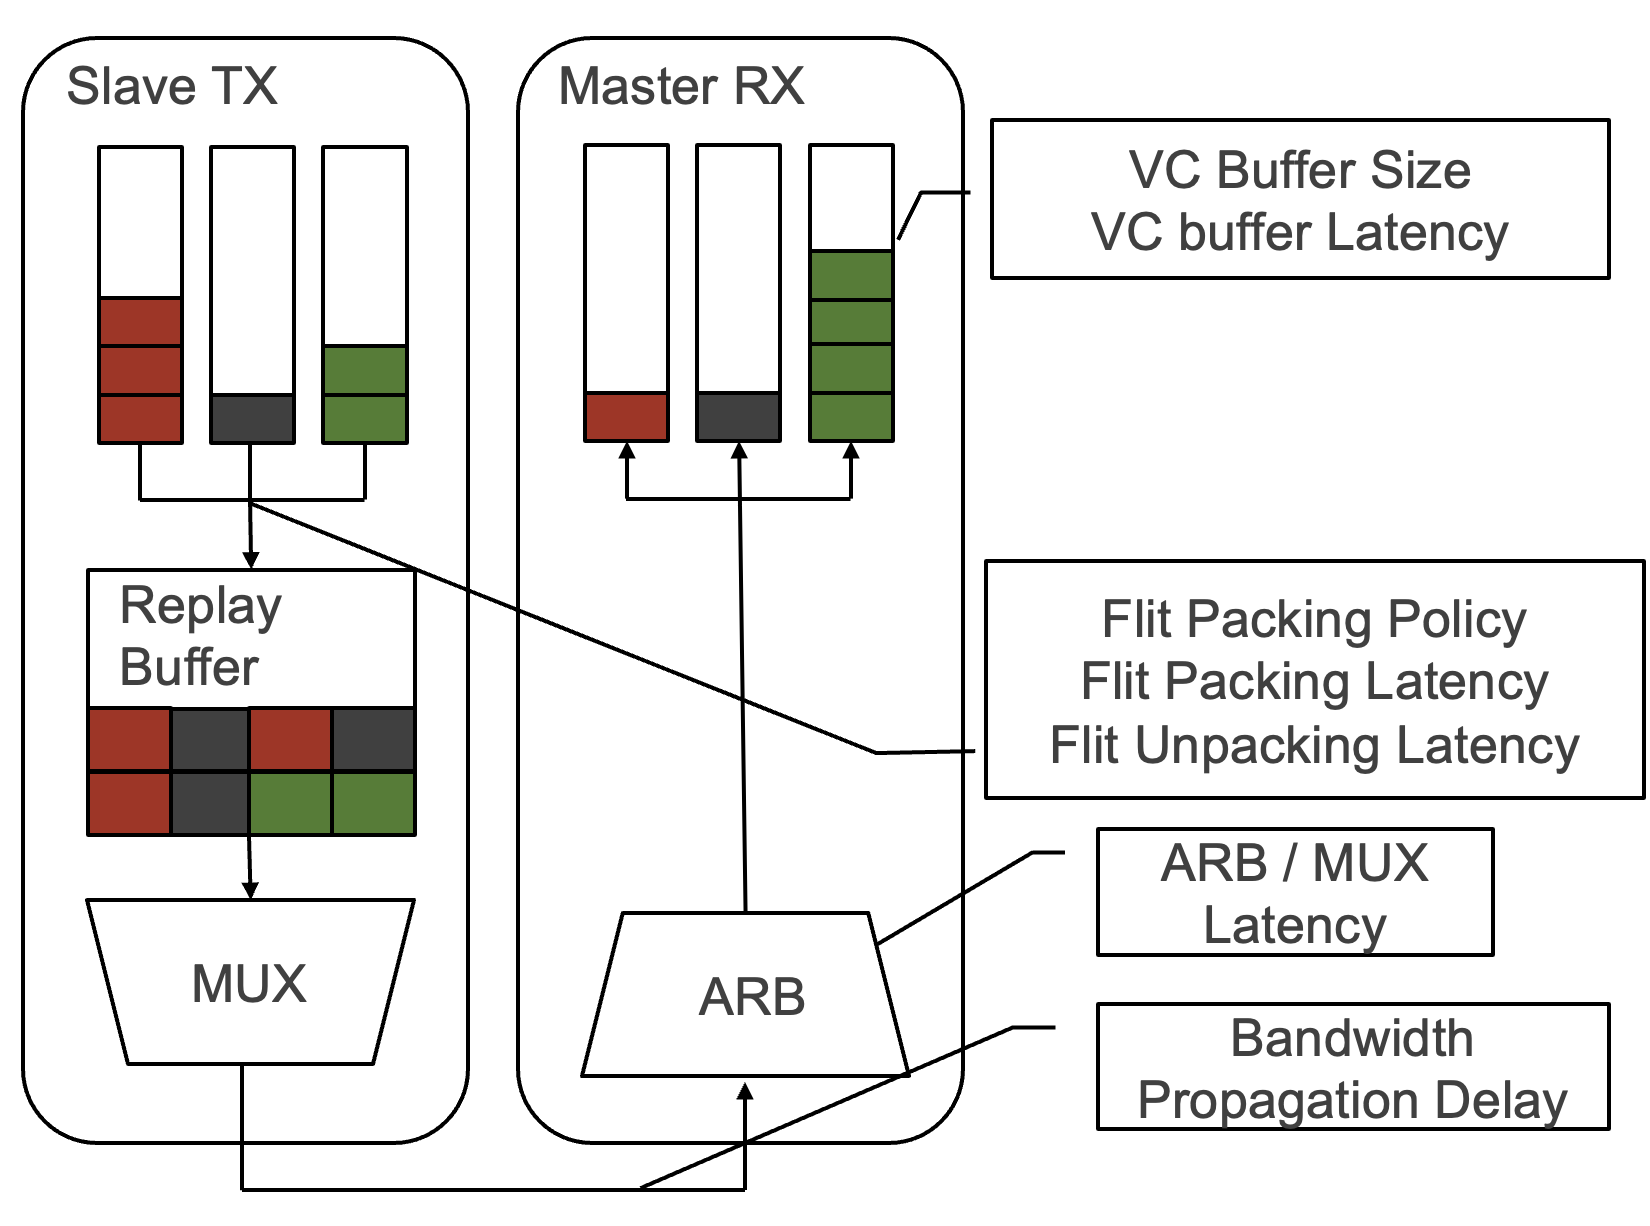
\includegraphics[width=\textwidth]{figures/cxlmem_timing_param.png}
  \caption{Major timing parameters in CXL interconnection.}
  \label{fig:cxlmem_timing_param}
\end{figure}
